\documentclass{beamer}

\usetheme{EastLansing}
%\usecolortheme{default}
%\usefonttheme{default}

\usepackage[english]{babel}
%\usepackage[francais]{babel}
\usepackage{graphicx, float}
\usepackage{subcaption}
\usepackage{pstool}
\usepackage{epstopdf}

%maths
\usepackage{amsmath}
\usepackage{amssymb}

%code
\usepackage{listings}

\usepackage{tikz}
\usepackage{pgfplots}
\usetikzlibrary{shapes,backgrounds}

%%%%%%%%%%%%%%%%%%%%%%%%%%%%%%%%%%%%%%%%%%%%%%%%%%%%%%%%%%%%%%%%%%%%%%%%%%%%%%
% \embedvideo{<poster or text>}{<video file (MP4+H264)>}
% \embedvideo*{...}{...}                     % auto-play
%%%%%%%%%%%%%%%%%%%%%%%%%%%%%%%%%%%%%%%%%%%%%%%%%%%%%%%%%%%%%%%%%%%%%%%%%%%%%%

\usepackage[bigfiles]{pdfbase}
\ExplSyntaxOn
\NewDocumentCommand\embedvideo{smm}{
  \group_begin:
  \leavevmode
  \tl_if_exist:cTF{file_\file_mdfive_hash:n{#3}}{
    \tl_set_eq:Nc\video{file_\file_mdfive_hash:n{#3}}
  }{
    \IfFileExists{#3}{}{\GenericError{}{File~`#3'~not~found}{}{}}
    \pbs_pdfobj:nnn{}{fstream}{{}{#3}}
    \pbs_pdfobj:nnn{}{dict}{
      /Type/Filespec/F~(#3)/UF~(#3)
      /EF~<</F~\pbs_pdflastobj:>>
    }
    \tl_set:Nx\video{\pbs_pdflastobj:}
    \tl_gset_eq:cN{file_\file_mdfive_hash:n{#3}}\video
  }
  %
  \pbs_pdfobj:nnn{}{dict}{
    /Type/RichMediaInstance/Subtype/Video
    /Asset~\video
    /Params~<</FlashVars (
      source=#3&
      skin=SkinOverAllNoFullNoCaption.swf&
      skinAutoHide=true&
      skinBackgroundColor=0x5F5F5F&
      skinBackgroundAlpha=0
    )>>
  }
  %
  \pbs_pdfobj:nnn{}{dict}{
    /Type/RichMediaConfiguration/Subtype/Video
    /Instances~[\pbs_pdflastobj:]
  }
  %
  \pbs_pdfobj:nnn{}{dict}{
    /Type/RichMediaContent
    /Assets~<<
      /Names~[(#3)~\video]
    >>
    /Configurations~[\pbs_pdflastobj:]
  }
  \tl_set:Nx\rmcontent{\pbs_pdflastobj:}
  %
  \pbs_pdfobj:nnn{}{dict}{
    /Activation~<<
      /Condition/\IfBooleanTF{#1}{PV}{XA}
      /Presentation~<</Style/Embedded>>
    >>
    /Deactivation~<</Condition/PI>>
  }
  %
  \hbox_set:Nn\l_tmpa_box{#2}
  \tl_set:Nx\l_box_wd_tl{\dim_use:N\box_wd:N\l_tmpa_box}
  \tl_set:Nx\l_box_ht_tl{\dim_use:N\box_ht:N\l_tmpa_box}
  \tl_set:Nx\l_box_dp_tl{\dim_use:N\box_dp:N\l_tmpa_box}
  \pbs_pdfxform:nnnnn{1}{1}{}{}{\l_tmpa_box}
  %
  \pbs_pdfannot:nnnn{\l_box_wd_tl}{\l_box_ht_tl}{\l_box_dp_tl}{
    /Subtype/RichMedia
    /BS~<</W~0/S/S>>
    /Contents~(embedded~video~file:#3)
    /NM~(rma:#3)
    /AP~<</N~\pbs_pdflastxform:>>
    /RichMediaSettings~\pbs_pdflastobj:
    /RichMediaContent~\rmcontent
  }
  \phantom{#2}
  \group_end:
}
\ExplSyntaxOff
%%%%%%%%%%%%%%%%%%%%%%%%%%%%%%%%%%%%%%%%%%%%%%%%%%%%%%%%%%%%%%%%%%%%%%%%%%%%%%

%couleurs du theme
\definecolor{Tauteur}{RGB}{0, 81, 40}
\definecolor{Ttitre}{RGB}{153, 194, 174}
\definecolor{Tdate}{RGB}{217, 232, 225}
\definecolor{Ttext}{RGB}{51, 51, 179}
\definecolor{Tsommaire}{RGB}{230, 240, 235}

\setbeamersize{text margin left=1cm,text margin right=1cm}


\setbeamertemplate{navigation symbols}{%personalisation de la bare
\insertslidenavigationsymbol % page
	% flèches: bouger d'une page, symb: inserer le no de page 
\insertframenavigationsymbol % frame
	% flèches: bouger d'une frame, symb: ?
\insertsubsectionnavigationsymbol % sous-section
	% flèches: bouger d'une sous-section, symb: ?
\insertsectionnavigationsymbol % section
	% flèches: bouger d'une section, symb: ?
}

%%%%%%%%%%%%% Python %%%%%%%%%%%%
% Default fixed font does not support bold face
\DeclareFixedFont{\ttb}{T1}{txtt}{bx}{n}{12} % for bold
\DeclareFixedFont{\ttm}{T1}{txtt}{m}{n}{12}  % for normal

% Custom colors
\usepackage{color}
\definecolor{deepblue}{rgb}{0,0,0.5}
\definecolor{deepred}{rgb}{0.6,0,0}
\definecolor{deepgreen}{rgb}{0,0.5,0}

% Python style for highlighting
\newcommand\pythonstyle{\lstset{
language=Python,
basicstyle=\ttm,
morekeywords={self},              % Add keywords here
keywordstyle=\ttb\color{deepblue},
emph={MyClass,__init__},          % Custom highlighting
emphstyle=\ttb\color{deepred},    % Custom highlighting style
stringstyle=\color{deepgreen},
frame=tb,                         % Any extra options here
showstringspaces=false
}}


% Python environment
\lstnewenvironment{python}[1][]
{
\pythonstyle
\lstset{#1}
}
{}

% Python for external files
\newcommand\pythonexternal[2][]{{
\pythonstyle
\lstinputlisting[#1]{#2}}}

% Python for inline
\newcommand\pythoninline[1]{{\pythonstyle\lstinline!#1!}}



\beamerboxesdeclarecolorscheme{blocQ}{Tauteur}{Ttitre}

\begin{document}
\title[MSPN]{TP 9 : Introduction to the Lattice Boltzmann Method}
\author{Lea Heiniger}
\date{12.05.2023}

% TITRE
\begin{frame}
\titlepage
\end{frame}

% equation
\section*{Theory and TP introduction}
\begin{frame}[fragile]
\frametitle{Lattice Boltzmann Method}
A method for fluid simulation based on the Lattice gas automata. This method can be used to numerically solve Navier-Stokes equations.\\
\bigskip
\begin{center}
\begin{large}
$\partial_{t}u-(u\cdot\nabla ) u = -\frac{1}{\rho_{0}}\nabla p+ \nu\nabla u$\\
$\nabla\cdot u=0$\\
\end{large}
\end{center}
with $u$ the velocity, $p$ the pressure and $\nu$ the viscosity
\end{frame}

\begin{frame}[fragile]
\frametitle{Lattice Boltzmann Method}
We simulate the \textbf{populations} of particles on a lattice and therefore we work with continuous values but time and space are still discrete.\\ %%%%% VELO ?
\bigskip\bigskip
Adventages over Lattice gas automata :\\
\begin{itemize}
\item Macroscopic scale\\
\item More particles can be simulated
\end{itemize}

% no more need to stay with integers, too much details (Lattice gaz automata), too much particles needed
\end{frame}

\begin{frame}[fragile]
\frametitle{D2Q9 model}
\vfill
Two dimensions and 9 directions (8 plus non-moving population)\\
\bigskip\bigskip\bigskip\bigskip
\begin{columns}[t]

\column{0.49\textwidth}
The value for each direction represents the \textbf{density} of particles going in that direction at that point.\\

\column{0.49\textwidth}
\begin{center}
\begin{figure}
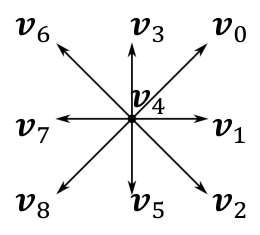
\includegraphics[width=0.45\textwidth]{img/d2q9.png}
\caption{vectors of the 9 possible directions}
\end{figure}
\end{center}

\end{columns}
\vfill
\end{frame}


\begin{frame}[fragile]
\frametitle{BGK Collision model}
\begin{center}
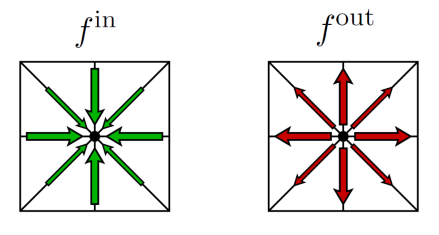
\includegraphics[width=0.6\textwidth]{img/col.png}\\
\bigskip
{\large $f_{i}^{out} =f_{i}^{in}-\omega\cdot (f_{i}^{in}-E(i,\rho , u))$}
\end{center}
\bigskip
With $E$ the local equilibrium
$E(i,\rho , u) = \rho t_{i} (1+\frac{\frac{\delta x}{\delta t}v_{i}\cdot u}{c_{s}^2}+\frac{1}{2c_{s}^{4}}(\frac{\delta x}{\delta t}v_{i}\cdot u)^{2}-\frac{1}{2c_{s}^2}\vert u\vert ^{2})$
\end{frame}

\begin{frame}[fragile]
\frametitle{Propagation}
Once $f_{i}^{out}$ computed we simply propagate every density to the point it is directed to in order to create $f_{i}^{in}$ for time $t+\delta t$\\
\bigskip
\begin{center}
\begin{large}
$ f_{i}^{in} = f_{i}^{out}(x-v_{i}\delta t, t-\delta t)$
\end{large}
\end{center}
\end{frame}


\begin{frame}[fragile]
\frametitle{Border outflows}
Since we work on a limited domain we have to take into account the populations going outside of the domain.\\
\bigskip\bigskip
therefore we apply outflows conditions :\\
\begin{python}
fin[col1,0,:] = fin[col1,1,:]
fin[col3,-1,:] = fin[col3,-2,:]
fin[lin1,:,0] = fin[lin1,:,1]
fin[lin3,:,-1] = fin[lin3,:,-2]
\end{python}
\end{frame}

\begin{frame}[fragile]
\frametitle{Perturbation function and initial parameters}
In order to simulate a Tornado we have to apply a perturbation at the center point at each time.\\
\begin{center}
\begin{large}
$\tilde{u}(t) = u_{LB}\begin{bmatrix}
           cos(\omega_{p}t) \\
           sin(\omega_{p}t)
         \end{bmatrix}$
\end{large}
\end{center}
With $u_{LB}$ the propagation speed and $\omega_{p}$ the pulse frequency\\
\bigskip\bigskip
We initialise the system at equilibrium (the velocity is null everywhere) and the density to 1
\end{frame}

\begin{frame}[fragile]
\frametitle{macroscopic quantities}
The density :\\
$\rho(x, t) = \displaystyle\sum_{i=0}^{8} f_{i}^{in}(x,t)$\\
\bigskip
The pressure :\\
$p = c_{s}^{2}\rho$\\
\bigskip
The velocity :\\
$u(x,t) = \frac{1}{\rho (x,t)}\frac{\delta x}{\delta t}\displaystyle\sum_{i=0}^{8}v_{i}f_{i}^{in}(x,t)$
\end{frame}


\section*{Results}

\begin{frame}[fragile]
\frametitle{Initial result}
With the initial values for $re$, $n_{x}$, $n_{y}$, $u_{LB}$ and $\omega_{p}=0.2$
\begin{figure}
\begin{subfigure}{0.48\textwidth}
\embedvideo{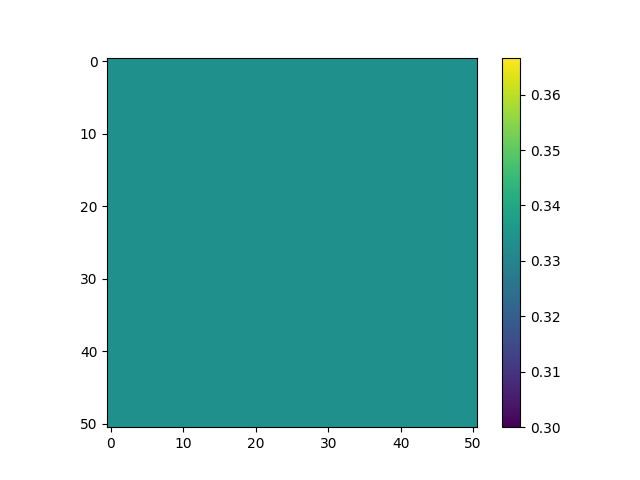
\includegraphics[width=\textwidth]{img/P_000.png}}{img/P_basic.mp4}
\caption{Pressure}
\end{subfigure}
\begin{subfigure}{0.48\textwidth}
\embedvideo{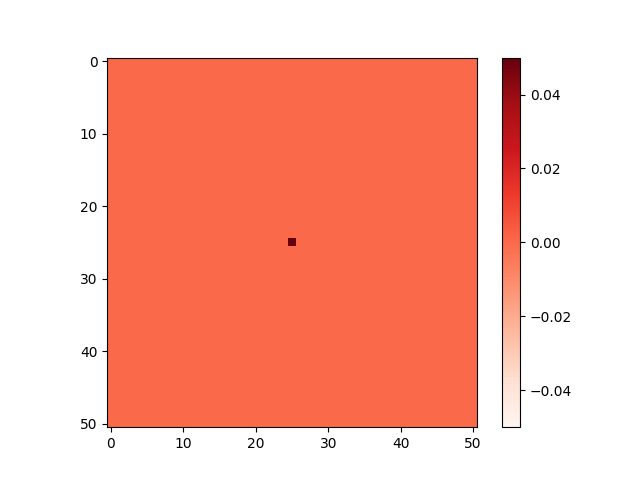
\includegraphics[width=\textwidth]{img/vel_000.png}}{img/vel_basic.mp4}
\caption{velocity}
\end{subfigure}
\end{figure}
\end{frame}

\subsection*{Parameters}
\begin{frame}[fragile]
\frametitle{the pulse frequency $\omega_{p}$}
% pulse frequency
\begin{figure}
\begin{subfigure}{0.48\textwidth}
\embedvideo{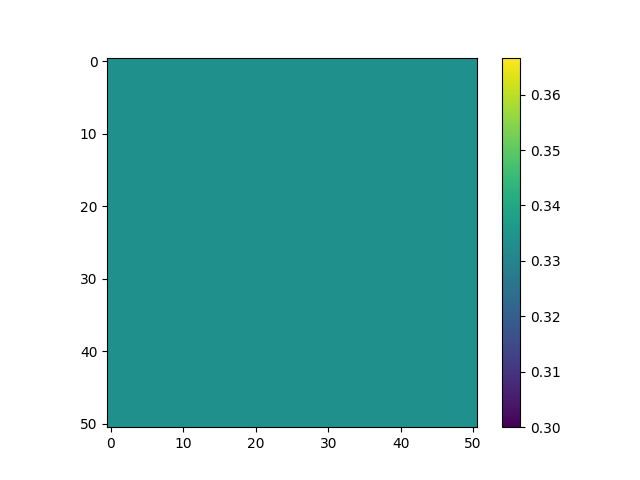
\includegraphics[width=\textwidth]{img/P_000.png}}{img/P_wp08.mp4}
\caption{$\omega_{p}=0.8$}
\end{subfigure}
\begin{subfigure}{0.48\textwidth}
\embedvideo{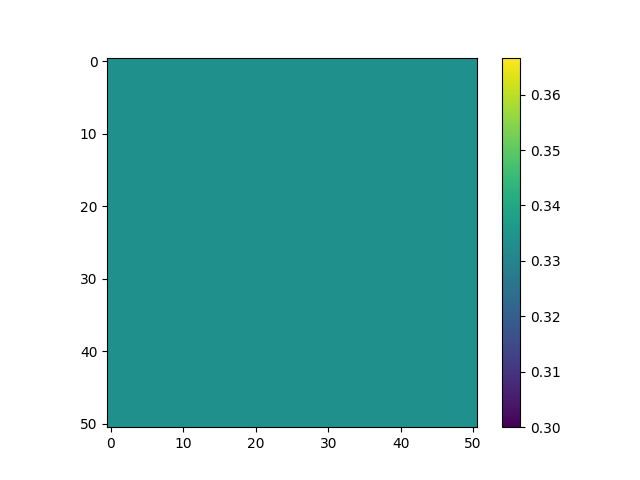
\includegraphics[width=\textwidth]{img/P_000.png}}{img/P_wp015.mp4}
\caption{$\omega_{p}=0.15$}
\end{subfigure}
\end{figure}
\end{frame}

\begin{frame}[fragile]
\frametitle{$n_{x},n_{y}$}
$n_{x}$ and $n_{y}$ define the size of the grid.\\
\begin{figure}
\begin{subfigure}{0.32\textwidth}
\centering
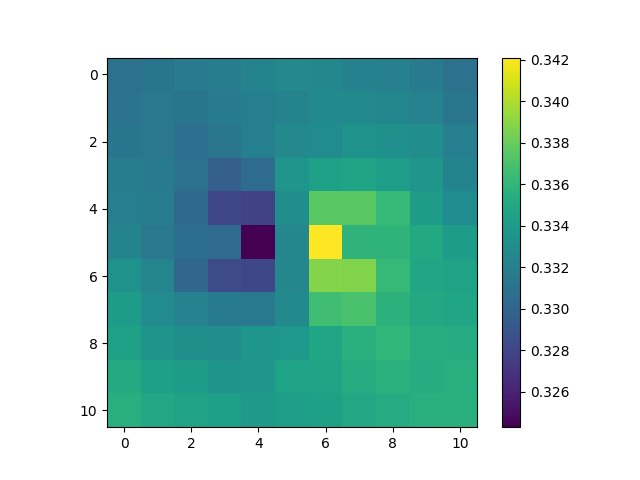
\includegraphics[width=\textwidth]{img/P_001_nxy11.png}
\caption{$n_{x}=n_{y}=11$}
\end{subfigure}
\begin{subfigure}{0.32\textwidth}
\centering
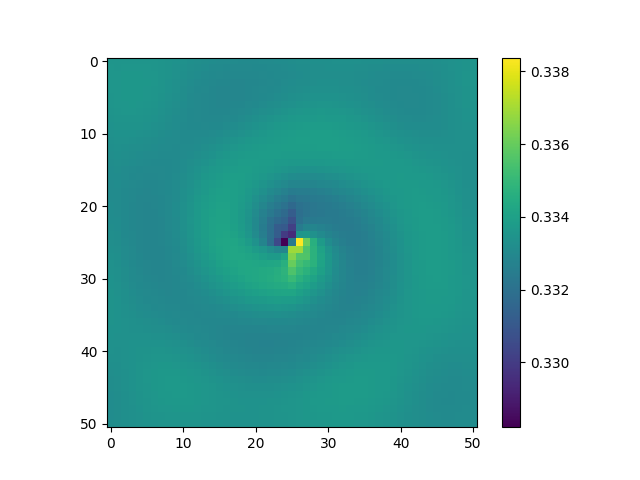
\includegraphics[width=\textwidth]{img/P_001_nxy51.png}
\caption{$n_{x}=n_{y}=51$}
\end{subfigure}
\begin{subfigure}{0.32\textwidth}
\centering
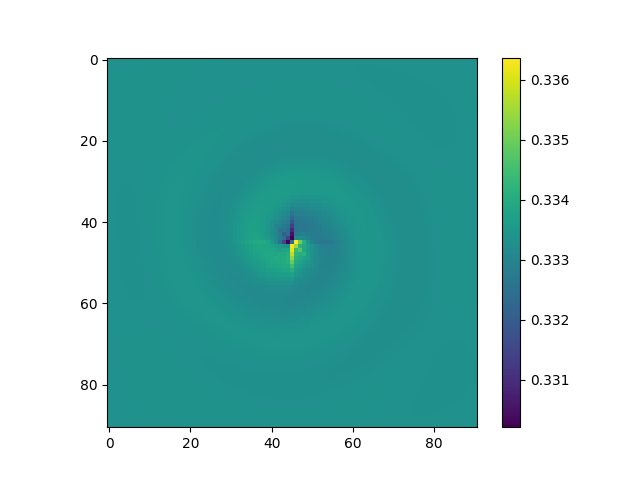
\includegraphics[width=\textwidth]{img/P_001_nxy91.png}
\caption{$n_{x}=n_{y}=91$}
\end{subfigure}
\end{figure}

\end{frame}


\begin{frame}[fragile]
\frametitle{Reynolds number $Re$}
$Re = \frac{UL}{\nu}$ is the ratio between the inertial forces and the viscous forces
\begin{figure}
\begin{subfigure}{0.48\textwidth}
\embedvideo{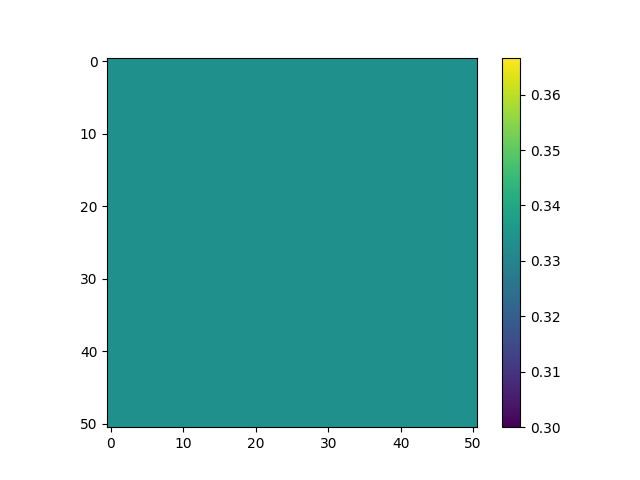
\includegraphics[width=\textwidth]{img/P_000.png}}{img/P_RE05.mp4}
\caption{$Re=5$}
\end{subfigure}
\begin{subfigure}{0.48\textwidth}
\embedvideo{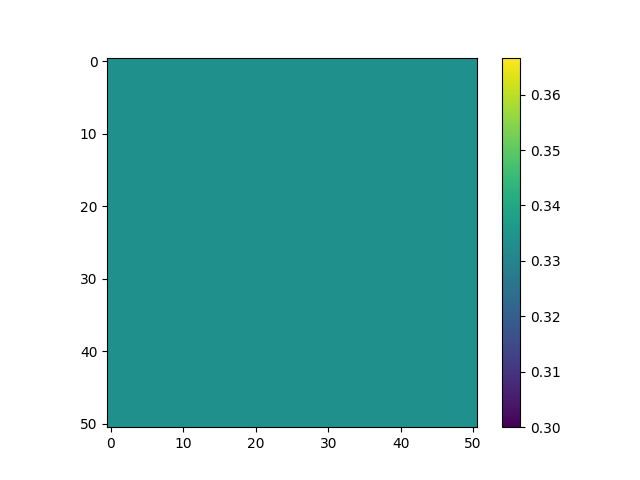
\includegraphics[width=\textwidth]{img/P_000.png}}{img/P_RE50.mp4}
\caption{$Re=50$}
\end{subfigure}
\end{figure}
\end{frame}

\begin{frame}[fragile]
\frametitle{$u_{LB}$}
$u_{LB}$ is the speed of propagation of the population. \\ 
It is related to the viscosity of the fluid.\\
\begin{figure}
\begin{subfigure}{0.48\textwidth}
\embedvideo{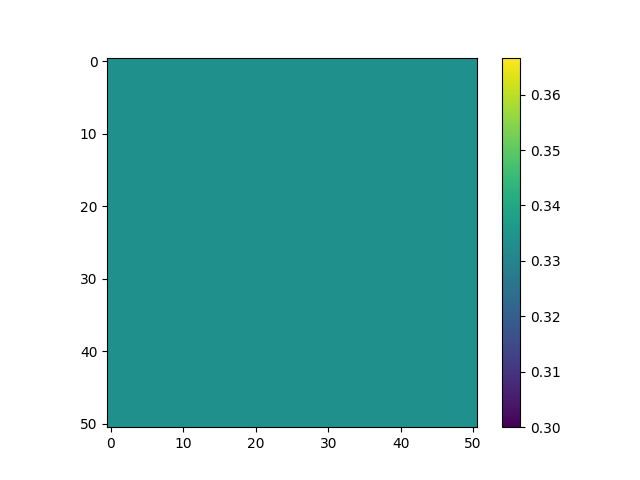
\includegraphics[width=\textwidth]{img/P_000.png}}{img/P_uLB01.mp4}
\caption{$u_{LB}=0.1$}
\end{subfigure}
\begin{subfigure}{0.48\textwidth}
\embedvideo{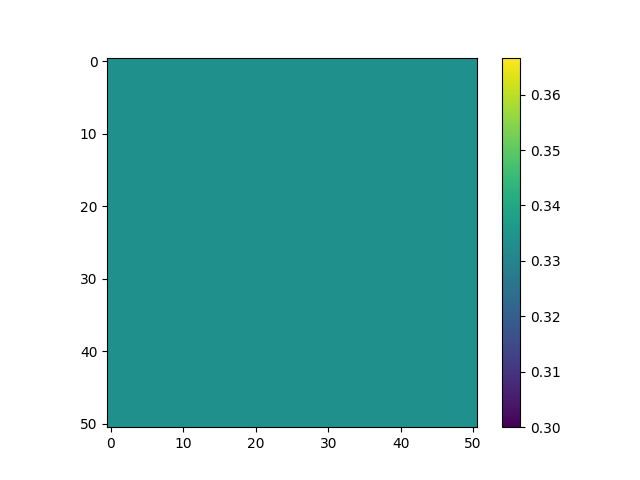
\includegraphics[width=\textwidth]{img/P_000.png}}{img/P_uLB0005.mp4}
\caption{$u_{LB}=0.005$}
\end{subfigure}
\end{figure}
\end{frame}

\subsection*{Moving center}

\begin{frame}[fragile]
\frametitle{Tornado center}

Whe introduce a new variable \texttt{center} that contains the coordinates of the tornado center on which we apply the perturbation.\\
\bigskip\bigskip
\begin{python}
center = array([int(nx/2), int(ny/2)])

for t in range(maxIter):
   ...
   u[:,center[0],center[1]] = perturbation(t)
   ...

\end{python}

\vfill
\end{frame}

\begin{frame}[fragile]
\frametitle{Outflow conditions}
\bigskip
When moving the center closer to one of the border we have to take into account the the outflow conditions conditions will have an impact.
\begin{center}
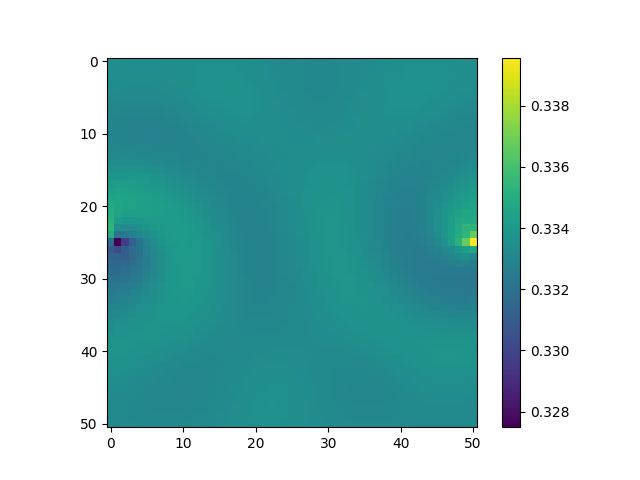
\includegraphics[width=0.7\textwidth]{img/border_conditions.png}

\end{center}

\end{frame}

\begin{frame}[fragile]
\frametitle{Linear trajectory}
One possibility is to move the center along a straight line.\\
\bigskip\bigskip

\begin{python}
center = array([int(nx/4),int(ny/4)])

for t in range(maxIter):
   ...
   u[:,center[0],center[1]] = perturbation(t)
   if time%80 == 0 : 
      center += 1
   ...

\end{python}

\vfill
\end{frame}

\begin{frame}[fragile]
\frametitle{Linear trajectory}
\begin{center}
\embedvideo{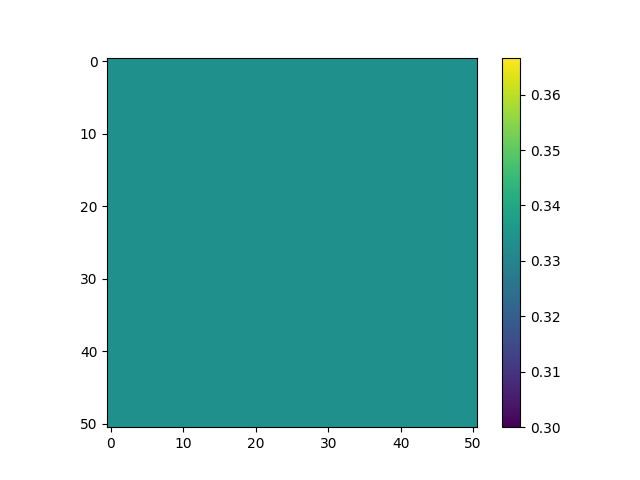
\includegraphics[width=0.8\textwidth]{img/P_000.png}}{img/P_diag.mp4}
\end{center}

\end{frame}

\begin{frame}[fragile]
\frametitle{Pressure determined trajectory}

A more realistic option is to move the center towards the lowest pressure at each iteration.\\
\bigskip\bigskip

\begin{python}
center = array([int(nx/2), int(ny/2)])

for t in range(maxIter):
   ...
   u[:,center[0],center[1]] = perturbation(t)
   c1, c2 = where(P==amin(P))
   center = array([c1[0], c2[0]])
   ...

\end{python}

\end{frame}

\begin{frame}[fragile]
\frametitle{Pressure determined trajectory}
\begin{center}
\embedvideo{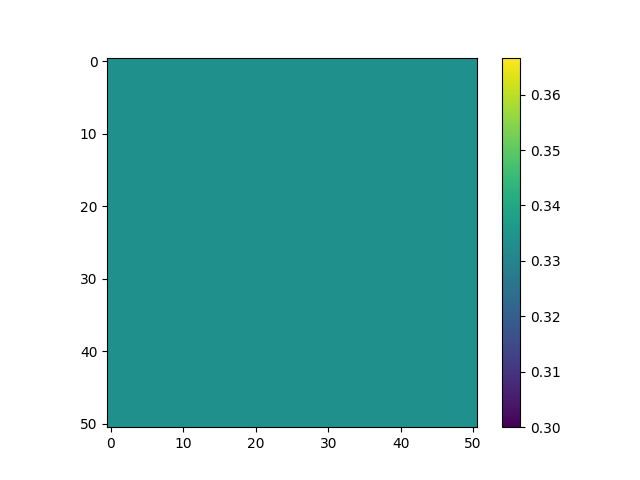
\includegraphics[width=0.8\textwidth]{img/P_000.png}}{img/P_pres.mp4}

\end{center}
\end{frame}

\end{document}
